\documentclass[a4paper,12pt]{article}

% --- Déclaration des packages 

\usepackage[utf8]{inputenc}
\usepackage[french]{babel}
\usepackage[T1]{fontenc}

\usepackage{amsmath}
\usepackage{amssymb}
\usepackage{mathrsfs}
\usepackage{stmaryrd}

\usepackage{tikz}
\usetikzlibrary{decorations.markings}
\usetikzlibrary{trees}
\usepackage{graphicx}

\usepackage{listings}
\lstset{language = bash, breaklines=true}
\usepackage{verbatim}
\usepackage{layout}
\usepackage[top=2.5cm, bottom=2.5cm, left=2.5cm, right=2.5cm]{geometry}

\usepackage{caption} % Pour ne pas avoir le "FIGURE - " qui traine sur les figures

\usepackage{tabularx} % Pour les tableaux

\usepackage[hidelinks]{hyperref} % Pour avoir les signets dans le PDF
\hypersetup{pdftex,colorlinks=false,allcolors=black}
\usepackage{hypcap}

\usepackage[nottoc,numbib]{tocbibind}
% --- Options de mise en page

\title{Rapport de stage 2A au Groupe Interdisciplinaire de Recherche en Éléments finis GIREF, Université Laval - Québec, CANADA}
\author{Grégoire MASSOT}
\date{15 Septembre 2015}

\pagestyle{plain} % ou headings ou empty

\setcounter{tocdepth}{3} % Niveau de précision de la table des matières

% --- Début du document

\begin{document}

\maketitle
\begin {figure}[!ht]
\begin{center}

\includegraphics [width =5cm]{LogoULaval.jpg}
\end{center}
\end{figure}

\begin {figure}[!ht]
\begin{center}

\includegraphics [width =5cm]{LogoEMSE.jpg}
\end{center}
\end{figure}
\newpage
\textbf{Dates du stage : } Du 22 Juin au 29 Août 2015 - 10 semaines

\textbf{Tuteur de stage Université Laval : } André FORTIN

\textbf{Tuteur École des Mines : } Julien BRUCHON
\tableofcontents
\newpage
\tikzset{->-/.style={decoration={
  markings,
  mark=at position #1 with {\arrow{>}}},postaction={destmaryrdcorate}}}
  
\section{Résolution d'une EDP par éléments finis de type Nédelec}
\subsection{Position du problème}
On travaille dans $\mathbb{R}^d$ avec $d=2$ ou $d=3$. On utilise le repère cartésien $(\vec{e_{x}}, \vec{e_{y}}, \vec{e_{z}})$ 
et les coordonnées cartésiennes usuelles $(x,y,z)$. Le domaine d'étude est noté $\Omega \subset \mathbb{R}^3$. 
Le problème que l'on cherche à résoudre sur $\Omega$ est le suivant :
\[
\vec{rot}(\vec{rot}(\vec{u}(x,y,z)) + \vec{u}(x,y,z) = \vec{f}(x,y,z)
\]
où $\vec{u}$ est le champ vectoriel que l'on cherche à déterminer et $\vec{f}$ est un champ connu, appelé "source".
\subsection{Formulation faible}
On prend une fonction test $\vec{v}(x,y,z)$ non identiquement nulle. 
On fait ensuite le produit scalaire de l'équation par $\vec{v}(x,y,z)$ et on intègre sur $\Omega$
\[
\int_{\Omega} {\vec{v}\cdot(\vec{rot}(\vec{rot}(\vec{u}) + \vec{u}) d\Omega} = \int_{\Omega} {\vec{v}.\vec{f} d\Omega}
\]

On va supposer que la solution $\vec{u}$ et la fonction test $\vec{v}$ sont dans l'espace de Hilbert suivant :
\[
V=H(rot, \Omega) =
\{ \vec{u} \in (\mathcal{L}^{2}(\Omega))^{3} \text{ tel que } \vec{rot}(\vec{u}) \in (\mathcal{L}^{2}(\Omega))^{3}
\}
\]

On va simplifier le terme en $\vec{rot}(\vec{rot}(u)) \cdot \vec{v}$. Une formule d'analyse vectorielle nous donne

\[
\vec{rot}(\vec{rot}(\vec{u})) \cdot \vec{v} = div(\vec{rot}(\vec{u}) \wedge \vec{v}) + \vec{rot}(\vec{u}) \cdot \vec{rot}(\vec{v})
\]

En notant $\wedge$ le produit vectoriel. Donc en intégrant sur le domaine $\Omega$
\begin{eqnarray*}
& &\int_{\Omega} {\vec{rot}(\vec{rot}(\vec{u})) \cdot \vec{v}} d\Omega = \int_{\Omega} {div(\vec{rot}(\vec{u}) \wedge \vec{v}) + \vec{rot}(\vec{u}) \cdot \vec{rot}(\vec{v})} d\Omega \\
&\Leftrightarrow& \int_{\Omega} {\vec{rot}(\vec{rot}(\vec{u})) \cdot \vec{v}} d\Omega = \int_{\partial \Omega} {(\vec{rot}(\vec{u}) \wedge \vec{v})\cdot\vec{n}} d\partial\Omega + \int_{\Omega} {\vec{rot}(\vec{u}) \cdot \vec{rot}(\vec{v})} d\Omega
\end{eqnarray*}
 Étant donné que $(\vec{rot}(\vec{u}) \wedge \vec{v}) \cdot \vec{n} = 
(\vec{n} \wedge \vec{rot}(\vec{u})) \cdot \vec{v} = 
(\vec{v} \wedge \vec{n}) \cdot \vec{rot}(\vec{u})$, le terme de bord va s'annuler si
$\vec{n} \wedge \vec{rot}(\vec{u}) = 0$ ou si $\vec{v} \wedge \vec{n}=0$.
La condition aux limites sera naturelle si $\vec{n} \wedge \vec{rot}(\vec{u}) = 0$ sur le bord
tandis qu'elle sera essentielle si $\vec{v}$ est choisie de sorte que $\vec{v} \wedge \vec{n}=0$ sur le bord.
Or $\vec{rot}(\vec{u}) \wedge \vec{n} = 0$ et $\vec{v}\cdot\vec{n}=0$ sur le bord donc on a $(\vec{rot}(\vec{u}) \wedge \vec{v})\cdot \vec{n} = 0$ sur le bord $\partial \Omega$.
On peut donc écrire la formulation variationnelle :

\[
\int_{\Omega} {\vec{rot}(\vec{u})\cdot\vec{rot}(\vec{v}) + \vec{u}\cdot\vec{v} d\Omega} = \int_{\Omega} {\vec{v}.\vec{f} d\Omega}
\]
La forme bilinéaire $a(\vec{u},\vec{v}) = \vec{rot}(\vec{u})\cdot\vec{rot}(\vec{v}) + \vec{u}\cdot\vec{v}$ est coercive
car elle correspond à la définition du produit scalaire dans $H(rot, \Omega)$. 
On peut donc appliquer le théorème de Lax-Milgram et avoir ainsi l'existence et l'unicité de la solution sur $H(rot, \Omega)$.
\subsection{Maillage du domaine et approximation de Galerkin}
\subsubsection{Espace d'approximation $V_{h}$}
On se place désormais dans le cas 2D.
Soit un maillage à $L$ triangles de notre domaine de travail $\Omega$ avec des éléments triangles $T^{l}$ 
numérotés par l'indice $l \in \llbracket 1,L \rrbracket$ et de taille inférieure à $h$.
On cherche la fonction $\vec{u}$ dans l'espace d'approximation conforme $V_{h}$ de $H(rot,\Omega)$
\[
V_{h} = {{\vec{v}_{h} \in H(rot, \Omega) \text{ tel que } \vec{v}_{h|T^{l}} \in \mathcal{R}^{1}(T^{l}) \forall l \in \llbracket 1,L \rrbracket}}
\]
avec $\forall l \in \llbracket 1,L \rrbracket$
\[\mathcal{R}^{1}(T^{l}) = \{ 
\vec{v_{h}}(x,y) = \vec{a} + \gamma
\begin{pmatrix}
-y\\
x
\end{pmatrix}
, \gamma \in \mathbb{R}
, \vec{a} \in \mathbb{R}^{2} 
\}\]

\subsubsection{Base de l'espace $V_{h}$}
Pour chaque triangle $l \in \llbracket 1,L \rrbracket$ de sommets $S_{1}^{l}$, $S_{2}^{l}$, $S_{3}^{l}$, on pose 3 fonctions \cite{ref2}

\[
\vec{\tau}_{i}^{l}(x,y)=\frac{1}{\det(\vec{S_{i+1}^{l} S_{i+2}^{l}},\vec{S_{i+1}^{l} S_{i}^{l}})}
\begin{pmatrix}
-y+y_{i+2}^{l} \\
x-x_{i+2}^{l}
\end{pmatrix}
\text{ sur } T^{l},\vec{0}\text{ ailleurs }
\]

Les $\vec{\tau_{i}^{l}}$ forment une base de l'espace d'approximation conforme $V_{h}$. On se concentre désormais sur un seul élément triangle d'indice $l=e$ 
noté $K_{e}$.
Ce triangle a ses arêtes orientées.

On peut alors écrire le champ inconnu $\vec{u}$ à l'intérieur de l'élément sous la forme de la combinaison 
linéaire des 3 champs vectoriels $\vec{\tau_{1}}(x,y)=\vec{\tau_{1}^{e}}(x,y)$, $\vec{\tau_{2}}(x,y)=\vec{\tau_{2}^{e}}(x,y)$ et $\vec{\tau_{3}}(x,y)=\vec{\tau_{3}^{e}}(x,y)$.
\begin{eqnarray*}
\vec{u}(x,y) &=& u_{1} \vec{\tau_{1}}(x,y) + u_{2} \vec{\tau_{2}}(x,y) + u_{3} \vec{\tau_{3}}(x,y)
\end{eqnarray*}
\subsubsection{Propriétés des fonctions de base}
Ces fonctions ont la propriété suivante :

\[
  \int_{A_{i}} {\vec{\tau}_{j}(x,y).\vec{t}_{i} ds} = 
  \left\{
  \begin{array}{r c l}
  \text{1 si i=j}\\
  \text{0 sinon}
  \end{array}
  \right.
\]

avec $ds$ l'élément de longueur et  $\vec{t}_{i}$ le vecteur unitaire tangent à l'arête $A_{i}$. Les fonctions de bases sont donc associées à une arête particulière.
Sur les 2 autres arêtes du triangle le champ est normal a l'arête
On peut donc écrire que pour $i \in \llbracket 1,3 \rrbracket$:

\begin{eqnarray*}
u_{i} &=& \int_{A_{i}} {\vec{u}(x,y).\vec{t_{i}} ds}\\
\end{eqnarray*}

Le coefficient $u_{i}$ est égal à l'intégrale le long de l'arête $A_{i}$ du produit scalaire $\vec{u}(x,y).\vec{t_{i}}$
\subsection{Construction du système matriciel élémentaire}
On va maintenant exprimer nos fonctions de base sur l'élément courant à partir des fonctions de base sur l'élément de référence
afin de pouvoir ramener toutes les intégrales qui constituent le système matriciel élémentaire à des intégrales sur l'élément de référence.
\subsubsection{Fonctions de base sur l'élément de référence}
On se place désormais sur l'élément de référence triangle $\hat{\Omega}$ avec le système de coordonnées $(\xi, \eta)$. 
Les sommets du triangle ont pour coordonnées $S_{1} (\xi = 0, \eta = 0)$, $S_{2} (\xi = 1, \eta = 0)$, $S_{3} (\xi = 0, \eta = 1)$
\begin{center}
\begin{tikzpicture}
  \draw[->] (0,0) -- (3,0);
  \draw[->] (0,0) -- (3,0) node[above] {$\xi$} coordinate (x axis);
  \draw[->] (0,0) -- (0,3) node[above] {$\eta$} coordinate (y axis);
  \draw (0,2) -- (2,0);
  \draw (0,0) node[below, left]{$S_{1}(0,0)$};
  \draw (0,2) node[left]{$S_{3}(0,1)$};
  \draw (2,0) node[below]{$S_{2}(1,0)$};
\end{tikzpicture}
\end{center}
Sur l'élement de référence, les fonctions de base s'écrivent de la façon suivante :

\begin{eqnarray*}
\vec{\tau_{1}^{ref}}(x,y) &=& (1-\eta,\xi)\\
\vec{\tau_{2}^{ref}}(x,y) &=& (-\eta,\xi)\\
\vec{\tau_{3}^{ref}}(x,y) &=& (-\eta,\xi-1)\\
\end{eqnarray*}

\begin{center}
\begin{figure}[h!]
\begin{tikzpicture}
\begin{scope}
\draw (0,0) -- (0,3) -- (3,0) -- (0,0);
\draw[->] (0,0.6) -- (1.2,0.6);
\draw[->] (0,1.2) -- (0.9,1.2);
\draw[->] (0,1.8) -- (0.6,1.8);
\draw[->] (0,2.4) -- (0.3,2.4);
\draw[->] (0.6,0) -- (2.1,0.3);
\draw[->] (1.2,0) -- (2.7,0.6);
\draw[->] (1.8,0) -- (3.3,0.9);
\draw[->] (2.4,0) -- (3.9,1.2);
\draw[->] (0.6,2.4) -- (0.9,2.7);
\draw[->] (1.2,1.8) -- (1.8,2.4);
\draw[->] (1.8,1.2) -- (2.7,2.1);
\draw[->] (2.4,0.6) -- (3.6,1.8);
\end{scope}
\begin{scope}[shift={(6,0)}]
\draw (0,0) -- (0,3) -- (3,0) -- (0,0);
\draw[->] (0,0.6) -- (-0.3,0.6);
\draw[->] (0,1.2) -- (-0.6,1.2);
\draw[->] (0,1.8) -- (-0.9,1.8);
\draw[->] (0,2.4) -- (-1.2,2.4);
\draw[->] (0.6,0) -- (0.6,0.3);
\draw[->] (1.2,0) -- (1.2,0.6);
\draw[->] (1.8,0) -- (1.8,0.9);
\draw[->] (2.4,0) -- (2.4,1.2);
\draw[->] (0.6,2.4) -- (-0.6,2.7);
\draw[->] (1.2,1.8) -- (0.3,2.4);
\draw[->] (1.8,1.2) -- (1.2,2.1);
\draw[->] (2.4,0.6) -- (2.1,1.8);
\end{scope}
\begin{scope}[shift={(12,0)}]
\draw (0,0) -- (0,3) -- (3,0) -- (0,0);
\draw[->] (0,0.6) -- (-0.3,-0.9);
\draw[->] (0,1.2) -- (-0.6,-0.3);
\draw[->] (0,1.8) -- (-0.9,0.3);
\draw[->] (0,2.4) -- (-1.2,0.9);
\draw[->] (0.6,0) -- (0.6,-1.2);
\draw[->] (1.2,0) -- (1.2,-0.9);
\draw[->] (1.8,0) -- (1.8,-0.6);
\draw[->] (2.4,0) -- (2.4,-0.3);
\draw[->] (0.6,2.4) -- (-0.6,1.2);
\draw[->] (1.2,1.8) -- (0.3,0.9);
\draw[->] (1.8,1.2) -- (1.2,0.6);
\draw[->] (2.4,0.6) -- (2.1,0.3);
\end{scope}
\end{tikzpicture}
\caption*{Les fonctions $\vec{\tau_{1}}(x,y)$, $\vec{\tau_{2}}(x,y)$ et $\vec{\tau_{3}}(x,y)$ sur l'élément de référence}
\end{figure}
\end{center}
\subsubsection{Transformation géométrique}
On a explicité les fonctions de bases sur un élément de référence. 
Il s'agit maintenant de savoir comment on passe de cet élément de référence à un 
élément ayant des sommets de coordonnées quelconques et des arêtes d'orientations quelconques.

\begin{center}
\begin{tikzpicture}
  \draw[->] (0,0) -- (3,0) node[right] {$\xi$} coordinate (x axis);
  \draw[->] (0,0) -- (0,3) node[above] {$\eta$} coordinate (y axis);
  \draw[->-=.5] (0,0) -- (2,0);
  \draw[->-=.5] (2,0) -- (0,2);
  \draw[->-=.5] (0,2) -- (0,0);
  
  \draw (0,0) node[below, left]{$S_{1,ref}(0,0)$};
  \draw (0,2) node[left]{$S_{3,ref}(0,1)$};
  \draw (2,0) node[below]{$S_{2,ref}(1,0)$};
  
  \draw[->] (2,2) to[bend left] (5,2);
  
  \draw[->] (6,0) -- (9,0) node[right] {$x$} coordinate (x axis);
  \draw[->] (6,0) -- (6,3) node[above] {$y$} coordinate (y axis);
  \draw[->-=.5] (7,2) -- (12,3);
  \draw[->-=.5] (12,3) -- (9,5);
  \draw[->-=.5] (7,2) -- (9,5);
  
  \draw (7,2) node[below]{$S_{1}(1,2)$};
  \draw (12,3) node[below]{$S_{2}(6,3)$};
  \draw (9,5) node[above]{$S_{3}(3,5)$};
\end{tikzpicture}
\end{center}

On définit une fonction 
\begin{eqnarray*}
\Psi : &\mathbb{R}^{2}& \rightarrow \mathbb{R}^{2} \\
&(\xi, \eta)& \rightarrow (x,y)
\end{eqnarray*}
qui à chaque sommet $i$ de l'élément de référence associe le sommet $i$ de l'élément courant. On peut aussi voir cette fonction comme un champ vectoriel sur l'ensemble du maillage.
Il est appelé dans MEF++ le "Champ de transformation géométrique". On va chercher ici une transformation linéaire, c'est à dire que l'on écrit :

\begin{eqnarray*}
x &=& a_{1} \xi + b_{1} \eta + c_{1} \\
y &=& a_{2} \xi + b_{2} \eta + c_{2} \\
\end{eqnarray*}

On résout ce système de 6 équations à 6 inconnues : 

\[
\left\{
\begin{array}{r c l}
f(S_{1, ref}) &=& S_{1} \\
f(S_{2, ref}) &=& S_{2} \\
f(S_{3, ref}) &=& S_{3} \\
\end{array}
\right.
\]

On obtient alors :

\[
\left\{
\begin{array}{r c l}
a_{1} &=&  x_{2} - x_{1}\\
b_{1} &=&  x_{3} - x_{1}\\
c_{1} &=&  x_{1}\\
\\
a_{2} &=&  y_{2} - y_{1}\\
b_{2} &=&  y_{3} - y_{1}\\
c_{2} &=&  y_{1}\\
\end{array}
\right.
\]
avec
\[
2\alpha = (x_{2} - x_{1})(y_{3}-y_{1}) - (x_{3} - x_{1})(y_{2}-y_{1})
\]
On en déduit la matrice jacobienne de $\Psi$

\[
J =
\begin{pmatrix}
\frac{\partial x}{\partial \xi} & \frac{\partial x}{\partial \eta} \\
\frac{\partial y}{\partial \xi} & \frac{\partial y}{\partial \eta} \\
\end{pmatrix}
=
\begin{pmatrix}
x_{2} - x_{1} & x_{3} - x_{1} \\
y_{2} - y_{1} & y_{3} - y_{1} \\
\end{pmatrix}
\]
On prend alors les formules suivantes pour la transformation des fonctions de base. Pour $i \in \llbracket 1,3 \rrbracket$
\begin{eqnarray*}
& &\vec{\tau}_{i}(x(\xi, \eta),y(\xi, \eta)) = (J^{-1})^{t}\vec{\tau}_{i}^{ref}(\xi, \eta) \\
& &\vec{rot}(\vec{\tau}_{i})(x(\xi, \eta),y(\xi, \eta)) = \frac{1}{det(J)}\vec{rot}(\vec{\tau}_{i}^{ref})(\xi, \eta)
\end{eqnarray*}
Celles ci sont démontrées dans l'annexe.
\subsubsection{Écriture des termes de formulation}
La fonction inconnue $\vec{u}$ et la fonction test $\vec{v}$ s'écrivent dans notre espace d'approximation interne $V_{h}$
\begin{eqnarray*}
\vec{u}(x,y) &=& u_{1} \vec{\tau_{1}}(x,y) + u_{2} \vec{\tau_{2}}(x,y) + u_{3} \vec{\tau_{3}}(x,y) \\
\vec{v}(x,y) &=& v_{1} \vec{\tau_{1}}(x,y) + v_{2} \vec{\tau_{2}}(x,y) + v_{3} \vec{\tau_{3}}(x,y)
\end{eqnarray*}
avec
\begin{eqnarray*}
\vec{\tau_{1}}(x,y) &=& \tau_{1,x}(x,y)\vec{e_{x}} + \tau_{1,y}(x,y)\vec{e_{y}} \\
\vec{\tau_{2}}(x,y) &=& \tau_{2,x}(x,y)\vec{e_{x}} + \tau_{2,y}(x,y)\vec{e_{y}} \\
\vec{\tau_{3}}(x,y) &=& \tau_{3,x}(x,y)\vec{e_{x}} + \tau_{3,y}(x,y)\vec{e_{y}}
\end{eqnarray*}
On écrit ces fonctions sous forme matricielle
\begin{equation*}
\vec{u}(x,y) =
\begin{pmatrix}
  \tau_{1,x} & \tau_{2,x} & \tau_{3,x}
\end{pmatrix}
\begin{pmatrix}
  u_{1} \\ u_{2} \\ u_{3}
\end{pmatrix}
\vec{e}_{x}
+
\begin{pmatrix}
  \tau_{1,y} & \tau_{2,y} & \tau_{3,y}
\end{pmatrix}
\begin{pmatrix} 
  u_{1} \\ u_{2} \\ u_{3}
\end{pmatrix}
\vec{e}_{y}
\end{equation*}

\begin{equation*}
\begin{split}
  \vec{v}(x,y) =
  \begin{pmatrix}
    \tau_{1,x} & \tau_{2,x} & \tau_{3,x}
  \end{pmatrix}
  \begin{pmatrix}
    v_{1} \\ v_{2} \\ v_{3}
  \end{pmatrix}
  \vec{e}_{x}
  +
  \begin{pmatrix}
    \tau_{1,y} & \tau_{2,y} & \tau_{3,y}
  \end{pmatrix}
  \begin{pmatrix}
    v_{1} \\ v_{2} \\ v_{3}
  \end{pmatrix}
  \vec{e}_{y}
  \\
  =
  \begin{pmatrix}
    v_{1} & v_{2} & v_{3}
  \end{pmatrix}
    \begin{pmatrix}
    \tau_{1,x} \\ \tau_{2,x} \\ \tau_{3,x}
  \end{pmatrix}
  \vec{e}_{x}
  +
  \begin{pmatrix}
    v_{1} & v_{2} & v_{3}
  \end{pmatrix}
    \begin{pmatrix}
    \tau_{1,y} \\ \tau_{2,y} \\ \tau_{3,y}
  \end{pmatrix}
  \vec{e}_{x}
  \vec{e}_{y}
\end{split} 
\end{equation*}

On écrit de même les rotationnels sous forme matricielle 

\begin{eqnarray*}
\vec{rot}(\vec{u}(x,y)) &=& 
u_{1} \vec{rot}(\vec{\tau_{1}}(x,y)) + u_{2} \vec{rot}(\vec{\tau_{2}}(x,y)) + u_{3} \vec{rot}(\vec{\tau_{3}}(x,y)) \\
&=& 
\begin{pmatrix}
(\frac{\partial \tau_{1,y}}{\partial x} - \frac{\partial \tau_{1,x}}{\partial y})
&
(\frac{\partial \tau_{2,y}}{\partial x} - \frac{\partial \tau_{2,x}}{\partial y})
&
(\frac{\partial \tau_{3,y}}{\partial x} - \frac{\partial \tau_{3,x}}{\partial y})
\end{pmatrix}
\begin{pmatrix}
  u_{1} \\ u_{2} \\ u_{3}
\end{pmatrix}
\vec{e}_{z}
\end{eqnarray*}

\begin{eqnarray*}
\vec{rot}(\vec{v}(x,y)) &=&
\begin{pmatrix} 
(\frac{\partial \tau_{1,y}}{\partial x} - \frac{\partial \tau_{1,x}}{\partial y})
&
(\frac{\partial \tau_{2,y}}{\partial x} - \frac{\partial \tau_{2,x}}{\partial y})
&
(\frac{\partial \tau_{3,y}}{\partial x} - \frac{\partial \tau_{3,x}}{\partial y})
\end{pmatrix}
\begin{pmatrix}
  v_{1} \\ v_{2} \\ v_{3}
\end{pmatrix}
\vec{e_{z}} \\
&=& 
\begin{pmatrix}
  v_{1} & v_{2} & v_{3}
\end{pmatrix}
\begin{pmatrix}
(\frac{\partial \tau_{1,y}}{\partial x} - \frac{\partial \tau_{1,x}}{\partial y}) 
\\
(\frac{\partial \tau_{2,y}}{\partial x} - \frac{\partial \tau_{2,x}}{\partial y})
\\
(\frac{\partial \tau_{3,y}}{\partial x} - \frac{\partial \tau_{3,x}}{\partial y})
\end{pmatrix}
\vec{e}_{z}
\end{eqnarray*}

La source $\vec{f}$ s'écrit :
\[
\vec{f}(x,y) =
f_{x}(x,y) \vec{e}_{x} + f_{y}(x,y) \vec{e}_{y}
\]

On revient à la formulation faible et on divise par $\begin{pmatrix} v_{1} & v_{2} & v_{3} \end{pmatrix}$. On obtient le système linéaire à 3 inconnues :
\[M^{e}U^{e} = F^{e}\]
avec
\begin{itemize}
\item $M^{e}$ la matrice masse $3\times3$
\item $F^{e}$ le vecteur résidu
\item $U^{e}$ le vecteur que l'on cherche
\end{itemize}

\begin{eqnarray*}
M^{e}_{i,j} &=& \int_{K_{e}} {\vec{\tau_{i}}.\vec{\tau_{j}} + \vec{rot}(\vec{\tau_{i}}).\vec{rot}(\vec{\tau_{j}}) dK_{e}} \\
&=&
\int_{\hat{\Omega}} {((J^{-1})^{t}\vec{\tau_{i}^{ref}}.(J^{-1})^{t}\vec{\tau_{j}^{ref}} + \frac{1}{\det(J)}\vec{rot}(\vec{\tau_{i}^{ref}}).\frac{1}{\det(J)}\vec{rot}(\vec{\tau_{j}^{ref}}))det(J) d\hat{\Omega}} \\
&=&
\int_{\hat{\Omega}} {\tilde{M}_{i,j} d\hat{\Omega}} \\
F^{e}_{i} &=&
\int_{K_{e}} {\vec{f_{i}}.\vec{\tau_{i}} dK_{e}} \\
&=&
\int_{\hat{\Omega}} {(\vec{f_{i}}.(J^{-1})^{t}\vec{\tau_{i}^{ref}}) det(J) d\hat{\Omega}} \\
&=&
\int_{\hat{\Omega}} {\tilde{F}_{i} d\hat{\Omega}} \\
\end{eqnarray*}
\subsubsection{Intégration numérique}
Enfin, on calcule les intégrales en faisant une quadrature de Hammer.
On intègre des polynomes d'ordre maximum 2.
On choisit donc un nombre $p$ de points d'intégrations supérieur à 3 :
\begin{eqnarray*}
M_{i,j} &=& \int_{\hat{\Omega}} {\tilde{M}_{i,j} d\hat{\Omega}}
= \sum_{k=1}^{p} W_{k} \tilde{M}_{i,j}(\xi_{k}, \eta_{k})
\\
F_{i} &=& \int_{\hat{\Omega}} {\tilde{F}_{i} d\hat{\Omega}}
= \sum_{k=1}^{p} W_{k} \tilde{F}_{i}(\xi_{k}, \eta_{k})
\end{eqnarray*}

\subsection{Assemblage et résolution}
\subsubsection{Assemblage}
On va ensuite créer ce système élémentaire pour chaque élément (ici des triangles) du maillage. 
Il s'agit ensuite de superposer les systèmes linéaires élémentaires pour obtenir notre système linéaire global.

On commence par numéroter les arêtes dans le maillage global $k=1..n$ et les orienter afin de les identifier. 
Le triangle d'indice $l$ a les arêtes d'indices $k_{l1},k_{l2},k_{l3}$. Le terme de la matrice de masse élémentaire
$M_{i,j}^{e}$ va être ajouté dans la case $M_{k_{li}, k_{lj}}$ et celui du vecteur résidu élémentaire $F_{i}^{e}$ va être ajouté à la case $F_{k_{li}}$
\subsubsection{Visualisation des résultats}
On fait le test sur un carré avec les sommets de coordonnées $(0,0)$, $(0,1)$, $(1,1)$, $(1,0)$. On utilise la solution analytique suivante
\[
\vec{u}(x,y)=
\begin{pmatrix}
2sin(\pi x)cos(\pi y) \\
cos(\pi x)sin(\pi y)
\end{pmatrix}
\]
Ce qui conduit à la source suivant :
\[
\vec{f}(x,y)=
\begin{pmatrix}
(\pi^{2}+2)sin(\pi x)cos(\pi y) \\
(1-\pi^{2})cos(\pi x)sin(\pi y)
\end{pmatrix}
\]
Après résolution, on obtient un vecteur solution de taille le nombre $n$ d'arêtes. Celui ci n'est pas exploitable en lui-même pour visualiser la solution. 
Il faut, pour chaque élément, calculer le champ sur quelques points de l'élément en reprenant la formule :
\begin{eqnarray*}
\vec{u}(x,y) &=& u_{k_{l1}} \vec{\tau_{k_{l1}}}(x,y) + u_{k_{l2}} \vec{\tau_{k_{l2}}}(x,y) + u_{k_{l3}} \vec{\tau_{k_{l3}}}(x,y) \text{ sur le triangle } l
\end{eqnarray*}
On fait donc une réinterpolation d'un champ \texttt{v3dnedelec} vers un champ \texttt{Vectoriel3D} dans MEF++.

\begin{figure}[h!]
\begin{center}
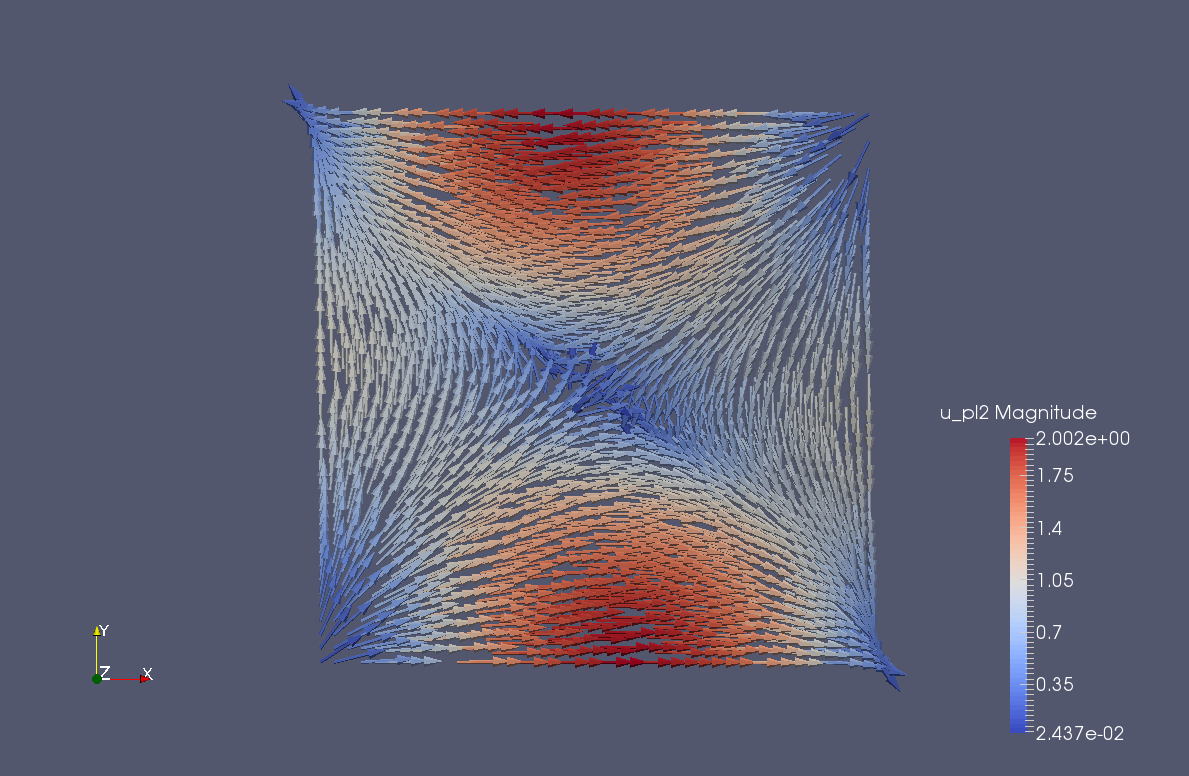
\includegraphics[scale=0.3]{carre_nedelec.png}
\caption*{Solution obtenue par éléments finis}
\end{center}
\end{figure}
\subsubsection{Étude de convergence $\mathcal{L}^{2}$}
On veut calculer la norme $\mathcal{L}^{2}$ de la différence entre le vecteur solution éléments finis et le vecteur solution analytique. 
\[
e_{\mathcal{L}^{2}} = \sqrt{\int_{\Omega} {(u-u_{sol})^{2} d{\Omega}}}
\]
Il faut pour cela que la solution analytique donnée plus haut soit comparable à la solution éléments finis. Il faut donc faire une réinterpolation du champ
\texttt{Vectoriel3D} vers \texttt{v3dnedelec} dans MEF++ avec la formule :
\begin{eqnarray*}
u_{i}^{sol} &=& \int_{A_{i}} {\vec{u}(x,y).\vec{t_{i}} ds}\\
\end{eqnarray*}
On obtient alors le tableau de convergence suivant.
\begin{center}
\begin{tabular}{|c|c|}
\hline
$h$ & $e_{\mathcal{L}^{2}}(h)$ \\
\hline
$5 \cdot 10^{-2}$ & 0.64 \\
\hline
$2.5 \cdot 10^{-2}$ &  0.32 \\
\hline
$1.25 \cdot 10^{-2}$ &  0.16 \\
\hline
\end{tabular}
\end{center}
On a donc une convergence à l'ordre 1 de $\vec{u}$
\subsection{Remarques}
\begin{itemize}
\item Le nombre de degrés de libertés est égal au nombre d'arêtes dans le maillage. C'est pour cela que l'on appelle les éléments de Nédelec des éléments d'arêtes.
\item On peut généraliser au cas 3D  avec des éléments tétraèdres. On a alors 6 arêtes par éléments. On a toujours une convergence de $\vec{u}$ à l'ordre 1
\item L'intérêt des éléments de Nédelec est de pouvoir imposer facilement une condition au bord $\vec{u} \wedge \vec{n}=0$, c'est à dire imposer un champ normal au bord.
Il suffit d'imposer que les coefficients associés aux arêtes au bord soient nuls. C'est l'équivalent d'une condition de Dirichlet homogène pour les éléments de Lagrange. 
\end{itemize}
\newpage
\section{Résolution d'une EDP par éléments finis de type Raviart-Thomas en 3D}
Les éléments de Raviart-Thomas sont aux faces ce que les éléments de Nédelec sont aux arêtes.
\subsection{Position du problème}
On travaille dans $\mathbb{R}^3$, on utilise le repère cartésien $(\vec{e_{x}}, \vec{e_{y}}, \vec{e_{z}})$ 
et les coordonnées cartésiennes usuelles $(x,y,z)$. Le domaine d'étude est noté $\Omega \subset \mathbb{R}^3$. 
Le problème que l'on cherche à résoudre sur $\Omega$ est le suivant :
\[
\left\{
\begin{array}{r c l}
&\vec{p} &= -\vec{grad}(u) \\
&div(\vec{p}) &= f
\end{array}
\right.
\]
$\vec{p}$ et $u$ sont nos champs inconnus. On a un \emph{problème mixte}.
\subsection{Formulation faible}
On prend les fonctions test $\vec{q}(x,y,z)$ et $v(x,y,z)$ non identiquement nulles. 
On fait ensuite le produit scalaire de la première équation par $\vec{q}$, on multiplie la seconde par $v$ et on intègre sur $\Omega$
\[
\left\{
\begin{array}{r c l}
\int_{\Omega} {\vec{p}\cdot\vec{q} + \vec{grad}(u)\cdot\vec{q}  d\Omega} = 0 \\
\int_{\Omega} {v div(\vec{p})  d\Omega} = \int_{\Omega} {v f  d\Omega} \\
\end{array}
\right.
\]

On va supposer que la solution $u$ et sa fonction test $v$ sont dans l'espace de Hilbert $V=\mathcal{L}^{2}(\Omega)$ 
et que $\vec{p}$ et $\vec{q}$ sont dans l'espace de Hilbert :
\[
Q = H(div, \Omega) = 
\{ \vec{p} \in (\mathcal{L}^{2}(\Omega))^{3} \text{ tel que }
div(\vec{p}) \in \mathcal{L}^{2}(\Omega)
\}
\]

On écrit la formulation variationnelle :
\[
\left\{
\begin{array}{r c l}
&&\int_{\Omega} {\vec{p}\cdot\vec{q} - u div(\vec{q}) d\Omega} = 0 \forall \vec{q} \in Q \\
\\
&&\int_{\Omega} {v div(\vec{p}) d\Omega} = \int_{\Omega} {v f d\Omega} \forall v \in V 
\end{array}
\right.
\]
Cette formulation variationnelle implique que $u=0$ sur $\partial \Omega$. En effet le théorème de la divergence nous donne
\[
\int_{\Omega} {\vec{grad}(u)\cdot\vec{q}  d\Omega} = \int_{\partial \Omega} {u \vec{q} \cdot \vec{n}  d\partial\Omega} -
\int_{\Omega} {u div(\vec{q}) d\Omega}
\]
Ceci montre que la condition de Dirichlet $u=0$ devient une condition naturelle pour la formulation variationnelle donnée.
\subsection{Maillage du domaine et approximation de Galerkin}
Soit un maillage à $L$ tétraèdres de notre domaine de travail $\Omega$ avec des éléments tétraèdres numérotés par l'indice $l \in \llbracket 1,L \rrbracket$ et de taille inférieure à $h$
On se concentre désormais sur un seul élément tétraèdre d'indice $l=e$ 
noté $K_{e}$.
Ce tétraèdre a ses faces orientées.

On peut alors écrire le champ inconnu $\vec{u}$ à l'intérieur de l'élément sous la forme de la combinaison 
linéaire des 4 champs vectoriels $\vec{\tau_{1}}(x,y,z)=\vec{\tau_{1}^{e}}(x,y,z)$, $\vec{\tau_{2}}(x,y,z)=\vec{\tau_{2}^{e}}(x,y,z)$,
$\vec{\tau_{3}}(x,y,z)=\vec{\tau_{3}^{e}}(x,y,z)$ et $\vec{\tau_{4}}(x,y,z)=\vec{\tau_{4}^{e}}(x,y,z)$
\begin{eqnarray*}
\vec{p}(x,y,z) &=& p_{1} \vec{\tau_{1}}(x,y,z) + p_{2} \vec{\tau_{2}}(x,y,z) + p_{3} \vec{\tau_{3}}(x,y,z) + p_{4} \vec{\tau_{4}}(x,y,z)
\end{eqnarray*}
Ces fonctions ont la propriété suivante :

\[
  \int_{F_{i}} {\vec{\tau}_{j}(x,y,z).\vec{n}_{i} dS} = 
  \left\{
  \begin{array}{r c l}
  \text{1 si i=j}\\
  \text{0 sinon}
  \end{array}
  \right.
\]

avec $\vec{n}_{i}$ le vecteur unitaire normal à la face $F_{i}$ et $dS$ l'élément d'aire de la face. Les fonctions de bases sont donc associées à une face particulière.
Sur les 3 autres faces du triangle le champ est tangent à la face.
On peut donc écrire que pour $i \in \llbracket 1,4 \rrbracket$:

\begin{eqnarray*}
p_{i} &=& \int_{F_{i}} {\vec{p}(x,y,z).\vec{n_{i}}(x,y,z) dS}\\
\end{eqnarray*}

Le coefficient $p_{i}$ est égal au flux sur la face $F_{i}$ de $\vec{p}(x,y,z)$
\subsection{Construction du système matriciel élémentaire}
\subsubsection{Fonctions de base sur l'élément de référence}
On se place désormais sur l'élément de référence tétraèdre $\hat{\Omega}$ avec le système de coordonnées $(\xi, \eta, \zeta)$. 
Les sommets du tétraèdre ont pour coordonnées $S_{1} (\xi = 0, \eta = 0, \zeta=0)$, $S_{2} (\xi = 1, \eta = 0, \zeta=0)$,
$S_{3} (\xi = 0, \eta = 1, \zeta=0)$, $S_{4} (\xi = 0, \eta = 0, \zeta=1)$.
\begin{center}
\begin{tikzpicture}
  \draw[->] (0,0) -- (3,0);
  \draw[->] (0,0,0) -- (0,0,3) node[above] {$\xi$} coordinate (x axis);
  \draw[->] (0,0,0) -- (3,0,0) node[above] {$\eta$} coordinate (y axis);
  \draw[->] (0,0,0) -- (0,3,0) node[above] {$\zeta$} coordinate (z axis);
  \draw (0,2,0) -- (2,0,0);
  \draw (0,0,2) -- (2,0,0);
  \draw (0,2,0) -- (0,0,2);
  \draw (0,0,2) node[left,below]{$S_{2}$};
  \draw (2,0,0) node[right,above]{$S_{3}$};
  \draw (0,2,0) node[right]{$S_{4}$};
  \draw (0,0,0) node[right, below]{$S_{1}$};
\end{tikzpicture}
\end{center}
Sur l'élément de référence, les fonctions de base s'écrivent de la façon suivante :
\begin{eqnarray*}
\vec{\tau_{1}^{ref}}(x,y,z) &=& (\xi,\eta,\zeta-1)\\
\vec{\tau_{2}^{ref}}(x,y,z) &=& (\xi,\eta-1,\zeta)\\
\vec{\tau_{3}^{ref}}(x,y,z) &=& (\xi,\eta,\zeta)\\
\vec{\tau_{4}^{ref}}(x,y,z) &=& (\xi-1,\eta,\zeta)
\end{eqnarray*}
\subsubsection{Transformation géométrique}
On généralise la transformation $\Psi$ et sa matrice jacobienne $J$ de la partie 1 à $\mathbb{R}^{3}$. 
On a alors les formules suivantes pour les transformations des fonctions de base du tétraèdre courant vers le tétraèdre de référence: 
\begin{eqnarray*}
& &\vec{\tau}_{i}(x(\xi, \eta, \zeta),y(\xi, \eta, \zeta), z(\xi, \eta, \zeta)) = \frac{J}{det(J)}\vec{\tau}_{i}^{ref}(\xi, \eta, \zeta) \\
& &div(\vec{\tau}_{i})(x(\xi, \eta, \zeta),y(\xi, \eta, \zeta), z(\xi, \eta, \zeta)) = \frac{1}{det(J)} div(\vec{\tau}_{i}^{ref})(\xi, \eta, \zeta)
\end{eqnarray*}
Ces formules sont démontrées dans l'annexe.
\subsubsection{Écriture des termes de formulation}
La fonction inconnue $\vec{p}$ et la fonction test $\vec{q}$ s'écrivent dans notre espace d'approximation interne $V_{h}$
\begin{eqnarray*}
\vec{p}(x,y) &=& p_{1} \vec{\tau_{1}}(x,y,z) + p_{2} \vec{\tau_{2}}(x,y,z) + p_{3} \vec{\tau_{3}}(x,y,z) + p_{4} \vec{\tau_{4}}(x,y,z) \\
\vec{q}(x,y) &=& q_{1} \vec{\tau_{1}}(x,y,z) + q_{2} \vec{\tau_{2}}(x,y,z) + q_{3} \vec{\tau_{3}}(x,y,z) + q_{4} \vec{\tau_{4}}(x,y,z)
\end{eqnarray*}
La fonction inconnue $u$ et sa fonction test $v$ sont constants sur l'élément. Après simplification de la première équation par $\begin{pmatrix} q1 & q2 & q3 \end{pmatrix}$,
et de la seconde équation par $v$, on obtient le système linéaire à 5 inconnues suivant : 
\[
\begin{pmatrix}
A^{e} & -(B^{e})^{t}\\
B^{e} & 0
\end{pmatrix}
\begin{pmatrix}
p\\
u
\end{pmatrix}
=
\begin{pmatrix}
0\\
f
\end{pmatrix}
\]
avec 
\begin{itemize}
 \item $A^{e}$ une matrice carrée $4 \times 4$
 \item $B^{e}$ un vecteur ligne $1 \times 4$
 \item $f^{e}$ un scalaire $1 \times 1$
\end{itemize}
\begin{eqnarray*}
A_{i,j}^{e} &=& \int_{K_{e}} {\vec{\tau_{i}}.\vec{\tau_{j}} dK_{e} } \\
&=&
\int_{\hat{\Omega}} {\frac{J}{det(J)}\vec{\tau_{i,ref}}.\frac{J}{det(J)}\vec{\tau_{j,ref}} det(J) \hat{d\Omega}} \\
&=&
\int_{\hat{\Omega}} {\tilde{A}_{i,j} d\hat{\Omega}} \\
B_{1,i}^{e} &=&
\int_{K_{e}} {div(\vec{\tau_{i}}) dK_{e}} \\
&=&
\int_{\hat{\Omega}} {\frac{1}{detJ}div(\vec{\tau_{i}^{ref}}) det(J) d\hat{\Omega}} \\
&=&
\int_{\hat{\Omega}} {\tilde{B}_{i} d\hat{\Omega}} \\
\end{eqnarray*}
Comme dans la partie 1, on calcule ces intégrales avec une quadrature de Hammer. On intègre des polynomes d'ordre maximum 2. 
On prend donc au minimum $p=4$ points d'intégration.
\subsection{Assemblage et résolution}
\subsubsection{Assemblage}
On assemble la matrice $A$ comme on assemblait la matrice $M$ dans la partie 1 par analogie entre les arêtes et les faces. 
Pour chaque tétraèdre $i \in \llbracket 1,n \rrbracket$ et ses 4 faces $F_{i_{j}}$ d'indice global $i_{j},j \in \llbracket 1,4 \rrbracket$ on pose : 
\[
  \left\{
  \begin{array}{r c l}
  & B_{i,i_{j}}=B_{1,j}^{e}\\
  & \text{ puis }0\text{ pour le reste de la ligne $i$}
  \end{array}
  \right.
\]
\subsubsection{Visualisation des résultats}
On fait le test sur un cube de sommets $(0,0,0)$, $(0,1,0)$, $(1,1,0)$, $(1,0,0)$, $(0,0,1$, $(0,1,1)$, $(1,1,1)$, $(1,0,1)$. 
On utilise la solution analytique suivante : 
\begin{eqnarray*}
u(x,y,z) &=& sin(\pi x)sin(\pi y)sin(\pi z) \\
\vec{p}(x,y,z) &=&
\begin{pmatrix}
-\pi cos(\pi x)sin(\pi y)sin(\pi z) \\
-\pi sin(\pi x)cos(\pi y)sin(\pi z) \\
-\pi sin(\pi x)sin(\pi y)cos(\pi z)
\end{pmatrix}
\end{eqnarray*}
Ce qui conduit au terme source suivant :
\[
f(x,y,z) = 3\pi^{2} sin(\pi x)sin(\pi y)sin(\pi z)
\]
Pour pouvoir visualiser le champ $\vec{p}$ obtenu par éléments finis, on fait une réinterpolation d'un champ \texttt{v3draviart} vers un champ \texttt{Vectoriel3D}
\begin{figure}[h!]
\begin{center}
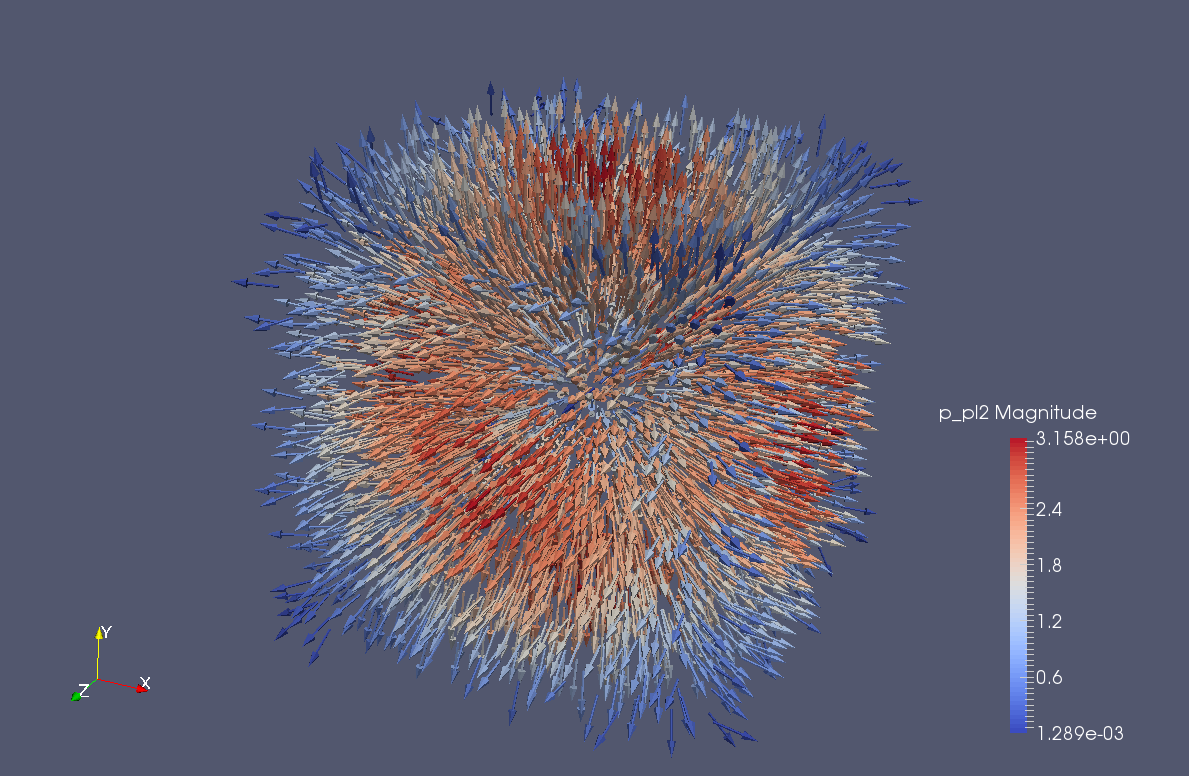
\includegraphics[scale=0.3]{cube_raviart.png}
\caption*{Solution $\vec{p}$ obtenue par éléments finis}
\end{center}
\end{figure}
\subsubsection{Étude de convergence $\mathcal{L}^{2}$}
Pour comparer la solution analytique $\vec{p_{sol}}$ à la solution obtenue par éléments finis, 
on fait un réinterpolation de $\vec{p_{sol}}$ d'un champ \texttt{Vectoriel3D} vers un champ \texttt{v3draviart}.
\begin{center}
\begin{tabular}{|c|c|c|}
\hline
$h$ & $e_{\vec{p},\mathcal{L}^{2}}(h)$ & $e_{u,\mathcal{L}^{2}}(h)$ \\
\hline
$25 \cdot 10^{-2}$ & 0.57 & 0.10\\
\hline
$12.5 \cdot 10^{-2}$ &  0.31 & 0.053\\
\hline
$6.125 \cdot 10^{-2}$ &  0.17 & 0.027\\
\hline
\end{tabular}
\end{center}
On a donc une convergence à l'ordre 1 en $\vec{p}$ et $u$
\newpage
\section{Aspects pratiques de l'utilisation de MEF++}
\subsection{A propos de MEF++}
Le logiciel MEF++ est développé depuis 1996 par le GIREF, une unité du département de mathématiques de l'Université Laval. 
Il est développé principalement par des ingénieurs et des professeurs d'université. 
Il est aussi développé par des doctorants et des stagiaires. MEF++ est développé à la fois pour la recherche publique et la recherche privée. 
Le laboratoire est donc financé à la fois par le CRSNG (un organisme public canadien) et par des entreprises.
\newline
\newline
MEF++ est principalement développé en C++. Il compte à ce jour 1.7 millions de lignes de code
\subsection{Principes généraux de la résolution d'une EDP sous MEF++}

Le choix de l'EDP à résoudre est fait à l'intérieur du code MEF++. Si on veut changer de problème, on change d'exécutable. 
En revanche le choix de $\Omega$, des conditions aux limites et des valeurs des champs connus sont lus par MEF++ depuis des fichiers externes.
\newline
\newline
On cherche à résoudre les EDP sur des objets quelconques. Par exemple un cube, une poutre, un tore. 
On commence par représenter cet objet avec une \emph{géométrie}. 
Ce sont les points, les courbes, les surfaces et les volumes qui permettent de se représenter l'objet dans l'espace.
Les points, les courbes, les surfaces et les volumes sont regroupés sous la notion de \emph{lieux géométriques}.
La \emph{géométrie} est donc l'ensemble des \emph{lieux géométriques} de notre objet. La géométrie est enregistrée dans un fichier \texttt{.geo}

On définit le \emph{maillage} à partir de la \emph{géométrie}. Il peut y avoir plusieurs \emph{maillages} par \emph{géométrie} mais un \emph{maillage} ne correspond qu'à une seule \emph{géométrie}. 
Les \emph{maillages} sont enregistrés au format \texttt{.mail}.

On définit ensuite les \emph{entités géométriques}. Ce sont des regroupements de \emph{lieux géométriques}. 
On définit souvent plusieurs \emph{entités géométriques} par \emph{géométrie}. Elles servent principalement à préciser sur quels bords on impose les conditions aux limites 
ou à définir les propriétés physiques des milieux.
Ils sont enregistrés sous le format \texttt{.enti}.

Les informations sur les champs qui sont en jeu dans l'EDP et les propriétés physiques des milieux sont enregistrées dans un fichier \texttt{.champ}

Les conditions aux limites sont définies dans le fichier \texttt{.CL}. Elles font références aux \texttt{.enti} et aux \texttt{.champs}.3
\newline
\newline
On crée le \texttt{.geo} à la main ou avec GMSH. On le passe dans GMSH pour obtenir un maillage au format \texttt{.unv}. 
On passe le \texttt{.unv} dans iMEF++ pour créer les entités géométriques et obtenir un \texttt{.mail} et un \texttt{.enti}
On code à la main le \texttt{.champs} et le \texttt{.CL} ou on les récupère à partir de templates.
\subsection{Organisation du répertoire de travail}
\subsubsection{Arborescence du répertoire de travail}
\begin{center}
\tikzstyle{every node}=[draw=black,thick,anchor=west]
\tikzstyle{selected}=[draw=red,fill=red!30]
\tikzstyle{optional}=[dashed,fill=gray!50]
\begin{figure}[h!]
\begin{tikzpicture}[%
  grow via three points={one child at (0.5,-0.7) and
  two children at (0.5,-0.7) and (0.5,-1.4)},
  edge from parent path={(\tikzparentnode.south) |- (\tikzchildnode.west)}]
  \node {mefpp\_gmassot}
    child { 
      node {GIREF}
      child { node {app}}
      child { node {bin}}
      child { node {lib}}
      child { node {scripts}}
      child { node {src}}
    }
    child [missing] {}				
    child [missing] {}				
    child [missing] {}	
    child [missing] {}	
    child [missing] {}	
    child {node {Tests\_probRaviart}}
    child {node {Tests\_probLaplacienVect}}
    child { 
      node {Tests\_probMaxwell}
	child { 
	  node {cube\_1}
	  child { node {div2}
	    child {node {cube.mail}}}
	  child [missing] {}	
	  child { node {div4}}
	  child { node {div8}}
	  child { node {cube.champs}}
	  child { node {cube.CL}}
	  child { node {cube.enti}}
	  child { node {launch\_probMaxwell.sh}}
	}
	child [missing] {}	
	child [missing] {}	
	child [missing] {}	
	child [missing] {}	
	child [missing] {}	
	child [missing] {}	
	child [missing] {}	
	child [missing] {}	
	child { node {carre\_1}}
	child { node {tetra\_1}}	
    }
    child [missing] {}	
    child [missing] {}	
    child [missing] {}	
    child [missing] {}	
    child [missing] {}	
    child [missing] {}	
    child [missing] {}	
    child [missing] {}	
    child [missing] {}	
    child [missing] {}	
    child [missing] {}	
    child { 
      node {maillages}
	child { 
	  node {cube\_1}
	  child { node {cube.geo}}
	  child { node {cube.mail}}
	  child { node {cube.unv}}
	}	
	child [missing] {}	
	child [missing] {}	
	child [missing] {}	
	child {node {carre\_1}}	
	child {node {tetra\_1}}		
    }
    ;
\end{tikzpicture}
\caption*{Arborescence du répertoire de travail personnel \texttt{mefpp\_gmassot}}
\end{figure}
\end{center}

\subsubsection{Dossier \texttt{GIREF/}}
Le dossier \texttt{GIREF/} contient le programme MEF++. C'est la copie du \emph{dépôt} Git. Il est composé de plusieurs dossiers :
\begin{itemize}
\item \texttt{app/} : contient des fichiers sources \texttt{.cc} ne contenant que des fonctions main. Une fonction main correspond à un exécutable et à une EDP particulière à résoudre.
\item \texttt{bin/} : contient les exécutables issus de ces fonctions main
\item \texttt{lib/} : contient les bibliothèques dynamiques \texttt{.so}. Ce sont ces outils qui sont appelés dans les fonctions main du dossier \texttt{app/}
\item \texttt{src/} : contient les sources dont sont issus les \texttt{.so}
\item \texttt{scripts/} : contient les scripts \texttt{.py} et \texttt{.sh} de routine (mise en forme des résultats exportés par exemple)
\end{itemize} 
\subsubsection{Dossier \texttt{maillages/} }

Le dossier \texttt{maillages/} contient les différents dossiers de maillages. Ce sont les dossiers de travail pour créer un \texttt{.unv} à partir d'un \texttt{.geo} avec GMSH.
On fait en sorte d'avoir des maillages grossiers en sortie de GMSH pour pouvoir les raffiner automatiquement avec l'outil \texttt{GIREF/bin/diviseAreteEn2} et ainsi faire des études de convergence.

\subsubsection{Dossier \texttt{Tests\_prob***/}}

On crée pour chaque problème un nouveau fichier main dans \texttt{GIREF/app/} et on crée un nouveau dossier générique dans la racine \texttt{mefpp\_gmassot} nommé
\texttt{Tests\_prob***/}. Par exemple \texttt{Tests\_probMaxwell/} correspond au premier problème étudié en partie 1, \texttt{Tests\_probRaviart/} correspond au second problème étudié en partie 2.

Dans chacun de ces dossiers, on copie les maillages du dossier \texttt{maillages/} qui nous intéressent, on crée des fichiers \texttt{.champs} et \texttt{.CL}
et on lance ensuite des scripts shell pour avoir une série de maillages de plus en plus fins et effectuer de manière automatique des tests de convergence sur une EDP.
\newline
\newline
On commence par créer des sous dossiers \texttt{div2/}, \texttt{div4/}, \texttt{div8/}...
Pour chaque sous-dossier \texttt{div\$i/}, on lance \texttt{GIREF/bin/diviseAreteEn2} et on met le résultat dans \texttt{../div\$i+1/}
On crée ensuite, dans chacun des sous-dossiers, un lien symbolique vers les fichiers \texttt{.enti}, \texttt{.CL}, \texttt{.champs}.

\begin{verbatim}
#!/bin/bash
mkdir div2
/home/mefpp_gmassot/GIREF/bin/diviseAreteEn2.opt cube div2/cube
for i in 2 4 8 16 32
do
mkdir -p div$i
cd div$i
ln -sf ../cube.{enti,CL,champs} .
cd ..
done

for i in 2 4 8 16
do
let "j = 2*i"
cd div$i
/home/mefpp_gmassot/GIREF/bin/diviseAreteEn2.opt cube ../div$j/cube
cd ..
done
\end{verbatim}
On peut ainsi lancer le programme à tester dans chaque dossier (par exemple \texttt{probMaxwell.opt})
\begin{verbatim}
for i  in 2 4 8 16 
do
cd  div$i
/home/mefpp_gmassot/GIREF/bin/probMaxwell.opt cube
cd ..
done
\end{verbatim}
On affiche dans chaque dossier les résultats importants qui ont été exportés par MEF++. Par exemple l'erreur en norme $\mathcal{L}^{2}$ entre la solution analytique
et la solution éléments finis.
\begin{verbatim}
for i in 2 4 8 16
do
cd div$i
cat NormeResiduL2.valeurs
cd ..
done 
\end{verbatim}
\subsection{Logiciels auxiliaires utilisés}
\subsubsection{Git}
Git est l'outil de gestion de version utilisé au GIREF. L'ensemble des fichiers sources, \emph{le dépôt}, est stocké sur un serveur.
On peut faire une copie du \emph{dépôt}, le modifier, puis faire un \emph{commit}, c'est à dire renvoyer les fichiers modifiés sur le serveur. 
Voici les principales commandes utilisées :

\begin{table}[!h]
\begin{center}
  \begin{tabularx}{\textwidth}{|c|X|}
  \hline
  \textbf{Commande Git} & \textbf{Fonction} \\
  \hline
  \texttt{git status} & Permet de voir l'ensemble des fichiers modifiés sur la copie du \emph{dépot} mais non commités. En vert les fichiers qui sont sur la liste du prochain \emph{commit}. En rouge les fichiers qui n'y sont pas \\
  \hline
  \texttt{git diff fichier} & Permet de voir les modifications faites sur \texttt{fichier} depuis le dernier \emph{commit} \\
  \hline
  \texttt{git add fichier} & Ajoute \texttt{fichier} sur la liste du prochain \emph{commit} \\
  \hline
  \texttt{git checkout (-p) fichier} & Enlève les modifications faites en local sur \texttt{fichier} \\
  \hline
  \end{tabularx}
\end{center}
\end{table}

On utilise aussi qGit qui est une interface graphique pour GIT. Elle permet de naviguer facilement entre les différents commits.
\subsubsection{Redmine}
Redmine est le gestionnaire de projet de MEF++. C'est un site web en interne qui contient, entre autres : 
\begin{itemize}
\item Une documentation : Elle est générée automatiquement à partir des commentaires des fichiers sources
\item Un wiki
\item Un fil d'actualité
\item Un forum
\end{itemize}

\subsubsection{Maple}

On utilise la méthode des solutions manufacturières pour tester les programmes. 
On a une solution connue de l'EDP et on en déduit le terme source à partir de cette EDP.
On utilise alors Maple afin de faire le calcul formel et rentrer l'expression du terme source dans le fichier \texttt{.champs}
Par exemple :
\begin{verbatim}
with(VectorCalculus)
Vx := 3*cos(Pi*x)*sin(Pi*y)*sin(Pi*z)
Vy := 2*sin(Pi*x)*cos(Pi*y)*sin(Pi*z)
Vz := sin(Pi*x)*sin(Pi*y)*cos(Pi*z)
v := VectorField(`<,>`(Vx, Vy, Vz), 'cartesian'[x, y, z])
champs := simplify(-Laplacian(v)+v)
\end{verbatim}

\subsubsection{Outils de parallelisation}
Le code MEF++ est parallélisé. On peut accélérer l'exécution des programmes en les lançant avec \texttt{mpirun}. 
On peut aussi les faire exécuter sur le centre de calcul de l'université \emph{Colosse}.
\newline
\newline
On peut aussi paralléliser la compilation des bibliothèques sur l'ensemble des machines du laboratoire avec l'outil \texttt{icecream}.
C'est utile quand on a tous les \texttt{.so} à recompiler.
\subsubsection{Autres logiciels}
Parmi les autres logiciels utilisés, on a :
\begin{itemize}
\item[$\bullet$] GMSH : c'est un mailleur libre et gratuit : \texttt{www.geuz.org/gmsh/}
\item[$\bullet$] Paraview : Il permet de visualiser les résultats obtenus sur la géométrie en 2D et en 3D
\item[$\bullet$] Vim : L'éditeur de texte pour modifier rapidement les fichiers \texttt{.champs}, les \texttt{.CL} et les scripts
\item[$\bullet$] QtCreator : un IDE complet et gratuit pour coder en C++
\item[$\bullet$] iMEF++ : un logiciel annexe à MEF++. Il sert principalement à créer des fichiers \texttt{.mail} et \texttt{.enti} à partir du fichier \texttt{.unv} issu de GMSH
\end{itemize}
\newpage
\section{Annexe : Démonstrations des transformations des fonctions de bases vers l'élément de référence}
On reprend la transformation $\Psi$ et sa matrice jacobienne $J$. On écrit la formule de Nanson \cite{ref} qui nous servira par la suite.
Elle donne la transformation d'un élément d'aire orienté $\vec{N}dA$ de $\hat{\Omega}$ en $\vec{n}da$ de $\Omega$
par $\Psi$ :
\[
\vec{n}da = det(J)(J^{-1})^{t}\vec{N}dA
\]
On travaille en dimension $n=2$ ou $n=3$. On note $(x_{1},...,x_{n})$  les coordonnées de l'espace courant et 
$(\hat{x}_{1},...,\hat{x}_{n})$ les coordonnées de l'espace de référence.
\subsection{Transformation des fonctions de bases de Nédelec}
Soit $\mathcal{C}$ un contour quelconque et $\hat{\mathcal{C}}$ sa transformation dans l'espace $\hat{\Omega}$.
On cherche un champ $\vec{u^{ref}}$ tel que :
\[
\int_{\mathcal{C}} {\vec{u}\cdot\vec{dr}} = \int_{\hat{\mathcal{C}}} {\vec{u^{ref}}\cdot\vec{dR}}
\]
On explicite le champ $\vec{u}\cdot\vec{dr}$ :
\begin{eqnarray*}
\vec{u}\cdot\vec{dr} &=& \sum_{j=1}^{n} {u_{j}dx_{j}} \\
&=& \sum_{j=1}^{n} \sum_{i=1}^{n} u_{j} \frac{\partial{x}_{j}}{\partial\hat{x}_{i}}d\hat{x}_{i} \\
&=& \sum_{i=1}^{n} \left( \sum_{j=1}^{n} u_{j} \frac{\partial{x}_{j}}{\partial\hat{x}_{i}} \right) d\hat{x}_{i} \\
&=& \sum_{i=1}^{n} u^{ref}_{i} d\hat{x}_{i}
\end{eqnarray*}
On en déduit que $u^{ref}_{i} = \sum_{j=1}^{n} u_{j} \frac{\partial{x}_{j}}{\partial\hat{x}_{i}}$ puis que $\vec{u^{ref}} = J^{t}\vec{u}$
. On en déduit ainsi que : 
$$\boxed{\vec{u} (x_{1},...,x_{n})= (J^{-1})^{t}\vec{u^{ref}}(\hat{x}_{1},...,\hat{x}_{n})}$$

\subsection{Transformation du rotationnel des fonctions de bases de Nédélec}
\subsubsection{En dimension 2}
On écrit le flux de $\vec{rot}(\vec{u})$ à travers $\Omega$. On utilise la formule de Green pour se ramener à une circulation sur le bord
$\partial \Omega$ : 
\[
\iint_{\Omega} {\vec{rot}(\vec{u}) \cdot \vec{e_{z}} d\Omega} = \int_{\partial \Omega}{\vec{u} \cdot d\vec{r}}
\]
On fait de même avec la fonction $\vec{u^{ref}}$
\[
\iint_{\hat{\Omega}} {\vec{rot}(\vec{u^{ref}}) \cdot \vec{e_{z}} d\hat{\Omega}} = \int_{\partial \hat{\Omega}}{\vec{u^{ref}} \cdot d\vec{R}}
\]
On utilise l'égalité des circulations de $\vec{u}$ sur $\mathcal{C}=\partial\Omega$ 
et de $\vec{u^{ref}}$ sur $\hat{\mathcal{C}} = \partial \hat{\Omega}$ du 4.1 pour écrire :
\[
\iint_{\Omega} {\vec{rot}(\vec{u}) \cdot\vec{e_{z}} d\Omega} = \iint_{\hat{\Omega}} {\vec{rot}(\vec{u^{ref}}) \cdot \vec{e_{z}} d\hat{\Omega}}
\]
On prend le membre de gauche et on se ramène à une intégrale sur $\hat{\Omega}$ avec la formule $d\Omega = det(J)d\hat{\Omega}$ :
\[
\iint_{\hat{\Omega}} {det(J) \vec{rot}(\vec{u}) \cdot \vec{e_{z}} d\hat{\Omega}} = \iint_{\hat{\Omega}} {\vec{rot}(\vec{u^{ref}}) \cdot \vec{e_{z}} d\hat{\Omega}}
\]
Ceci est vrai pour tout $\hat{\Omega}$. On en déduit la formule de transformation entre $\vec{rot}(\vec{u})$ et $\vec{rot}(\vec{u^{ref}})$
$$\boxed{\vec{rot}(\vec{u})(x_{1},x_{2}) = \frac{1}{det(J)}\vec{rot}(\vec{u^{ref}})(\hat{x}_{1},\hat{x}_{2})}$$
\subsubsection{En dimension 3}
On écrit le flux de $\vec{rot}(\vec{u})$ à travers $\mathcal{S} \in \partial \Omega$. On utilise la formule de Stokes pour se ramener à une circulation 
sur un contour $\mathcal{C}$ sur lequel s'appuie $\mathcal{S}$ : 
\[
\iint_{\mathcal{S}} {\vec{rot}(\vec{u}) \cdot \vec{n} da} = \int_{\mathcal{C}}{\vec{u} \cdot d\vec{r}}
\]
On fait de même avec la fonction $\vec{u^{ref}}$
\[
\iint_{\hat{\mathcal{S}}} {\vec{rot}(\vec{u^{ref}}) \cdot \vec{N}dA} = \int_{\hat{\mathcal{C}}}{\vec{u^{ref}} \cdot d\vec{R}}
\]
On utilise l'égalité des circulations de $\vec{u}$ sur $\mathcal{C}$ 
et de $\vec{u^{ref}}$ sur $\hat{\mathcal{C}}$ du 4.1 pour écrire :
\[
\iint_{\mathcal{S}} {\vec{rot}(\vec{u}) \cdot\vec{n} da} = \iint_{\hat{\mathcal{S}}} {\vec{rot}(\vec{u^{ref}}) \cdot \vec{N} dA}
\]
On prend le membre de gauche et on se ramène à une intégrale sur $\hat{\mathcal{S}}$ avec la formule de Nanson  :
en remarquant que $\vec{u} \cdot \left((J^{-1})^{t} \vec{N}\right) = \left(J^{-1} \vec{u}\right) \cdot \vec{N}$ : 
\[
\iint_{\hat{\mathcal{S}}} {J^{-1}det(J) \vec{rot}(\vec{u}) \cdot dA\vec{N}} = \iint_{\hat{\mathcal{S}}} {\vec{rot}(\vec{u^{ref}}) \cdot dA\vec{N}}
\]
Ceci est vrai pour tout $\hat{\mathcal{S}}$. On en déduit la formule de transformation : 
$$\boxed{\vec{rot}(\vec{u})(x_{1},x_{2},x_{3}) = \frac{J}{det(J)}\vec{rot}(\vec{u^{ref}})(\hat{x}_{1},\hat{x}_{2},\hat{x}_{3})}$$
\subsection{Transformation des fonctions de bases de Raviart-Thomas}
On se place désormais seulement dans le cas 3D. Soit $\mathcal{S}$ une surface quelconque et $\hat{\mathcal{S}}$ sa transformation dans l'espace $\hat{\Omega}$.
On cherche un champ $\vec{u^{ref}}$ tel que :
\[
\iint_{\mathcal{S}} {\vec{u}\cdot \vec{n} da} = \iint_{\hat{\mathcal{S}}} {\vec{u^{ref}}\cdot \vec{N}dA}
\]
On développe le terme de gauche avec la formule de Nanson en remarquant que $\vec{u} \cdot \left((J^{-1})^{t} \vec{N}\right) = \left(J^{-1} \vec{u}\right) \cdot \vec{N}$:
\[
\iint_{\hat{\mathcal{S}}} {\vec{u}\cdot det(J) (J^{-1})^{t} \vec{N} dA} = \iint_{\hat{\mathcal{S}}} {\vec{u^{ref}}\cdot \vec{N} dA}
\]
. On en déduit que :
\[
\iint_{\hat{\mathcal{S}}} {\left(det(J) J^{-1} \vec{u} - \vec{u^{ref}}\right) \cdot  \vec{N} dA} = 0
\]
Ceci est vrai pour toute surface $\hat{\mathcal{S}}$, donc
$$\boxed{\vec{u} (x_{1},x_{2},x_{3})= \frac{J}{det(J)}\vec{u^{ref}}(\hat{x}_{1},\hat{x}_{2},\hat{x}_{3})}$$
\subsection{Transformation de la divergence des fonctions de bases de Raviart-Thomas}
On écrit l'intégrale sur le volume $\Omega$ de $div(\vec{u})$. On utilise le théorème de la divergence
pour se ramener à un flux sur le bord $\partial \Omega$ :
\[
\iiint_{\Omega} {div(\vec{u}) d\Omega} = \iint_{\partial \Omega}{\vec{u} \cdot \vec{n}da}
\]
On fait de même avec la fonction $\vec{u^{ref}}$
\[
\iiint_{\hat{\Omega}} {div(\vec{u^{ref}}) d\hat{\Omega}} = \iint_{\partial \hat{\Omega}}{\vec{u^{ref}} \cdot \vec{N}dA}
\]
On a alors, d'après l'égalité de départ de 4.3 :
\[
\iiint_{\Omega} {div(\vec{u}) d\Omega} = \iiint_{\hat{\Omega}} {div(\vec{u^{ref}}) d\hat{\Omega}}
\]
On transforme le membre de gauche en utilisant la formule $d\Omega = det(J)d\hat{\Omega}$ :
\[
\iiint_{\hat{\Omega}} det(J) {div(\vec{u}) d\hat{\Omega}} = \iiint_{\hat{\Omega}} {div(\vec{u^{ref}}) d\hat{\Omega}}
\]
Ceci est vrai pour tout volume $\hat{\Omega}$. On en déduit la formule de transformation de la divergence :
$$\boxed{div(\vec{u}) (x_{1},x_{2},x_{3})= \frac{1}{det(J)}div(\vec{u^{ref}})(\hat{x}_{1},\hat{x}_{2},\hat{x}_{3})}$$
\newpage
\bibliographystyle{plain}
\bibliography{bibliographie}
\end{document}
